\chapter{Design and Implementation} %  Design Principles and Architecture
%TODO add chapter introduction

% - 5-10 pages
% - goal: fellow student understands content and would be able to more or less reproduce work
% - legitimate chosen approach
% - develop own ideas, trace them to existing theories
% - analysis and development
% - why was the approach (algorithm/technique/...) chosen and how does it work
% - show how concepts from theory are applied
% - test setup and achieved results

% possible steps:
% - requirement study
% - analysis / design -> UML, interaction, behavioural model, basic algorithms/methods, detailed description of models and their interactions (class/sequence diagrams)
% - manual, how to use program/device
% - system development and implementation

% ---

% considerations:
% - ipv6 not 100 percent necessary, but would be good
% - easy to learn
% - easy to adapt (to counterpart-interface updates) -> plug-in system?
% - tosca-orchestrator:
%   - 4.3ff of \url{http://docs.oasis-open.org/tosca/TOSCA-Instance-Model/v1.0/csd01/TOSCA-Instance-Model-v1.0-csd01.html#_Toc500843787}
%     "orchestrators manage the state of nodes and transitions them from state to state. This notion of state is somewhat artificial in that the orchestrator assumes a stable state is reached after an operation executes [...] without error"
%     "an error results in an undefined state" (no automatic rollback defined in tosca)
%     "orchestration states are only valid during orchestration. [...] the orchestrator or the imperative workflow [...] must decide the current state of all nodes in the topology.
%     "[...] event stream can be maintained for the life of a deployment [...]"
%     "As nodes are transitioned through their states, a subset of attributes and relationships may be defined. [...] This requires that in general TOSCA implies semantics such that not all attributes would be available in a given state."
%     "Nodes are only visible when they have a state defined (i.e. the orchestrator is dealing with their lifecycle)"
%     "node attributes are only defined for the stable states"
%     "node relationships are always navigable when the source and target node exists"
%     "[...] state is never updated outside an orchestration. [...] no way to propagate state changes from the node to the orchestrator and nodes don't have a state attribute."
%       -> no state file!
%     "Nodes can update their attributes with no specific guarantees in terms of precision or accuracy"

\section{Requirements}
The orchestrator should understand \gls{toscaacr}, extensions from it and should be able to provision bare-metal machines. Not only is it possible to split this into subtasks, but it makes sense as well. By doing so, the modules can be developed and updated one after another, in parallel if necessary and at a later point even interchanged with other implementations. In order to slice the application into reasonable packages, their domains should not overlap, and their external interface as small as possible.
\newline
To achieve that goal, the application workflow needs to be analyzed:
\newline
At the beginning, the \gls{csaracr} files, its content and the \gls{yamlacr} structure of the content needs to be parsed and validated. This includes handing down properties of both type-from-type and template-from-type derivations, as well as enabling (namespaced) imports.
Then, the orchestrator must be able to wake machines with \gls{wolacr}.
After a machine is powered on, it attempts to boot over network.
Therefore, the orchestrator has to manipulate an external or internal (as in \textquote{integrated in the orchestration software}) \gls{dhcpacr} server.
In order to provide the orchestrator with the necessary information about the machine, it makes sense to use a live-\gls{osacr} that does not need to be installed, but can be booted directly. Optimally, it should be relatively small, since its transferred via network, boot fast, and somehow provide the orchestrator with information about the underlying hardware like its RAM-size.
The last step is then running commands on the machine like installing a package or copying files to it. Optimally, the user should be informed on what is currently going on during the whole process.
\newline
Figure \ref{image:workflow} shows the whole workflow in an interaction overview diagram.

\begin{figure}[H]
  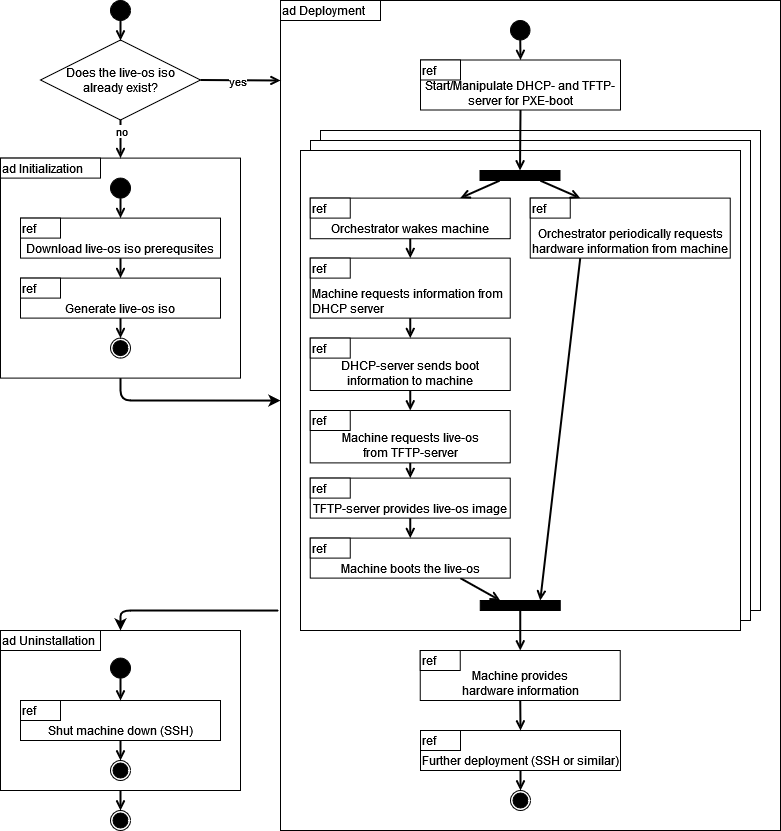
\includegraphics[width=14cm]{workflow}
  \centering
  \caption{UML interaction overview diagram describing the application workflow}
  \label{image:workflow}
\end{figure}

\section{Architecture}
To diminish the limitations of a web-based approach for the orchestrator like the hogging of resources even during idle times, the goal is to have one or many libraries, and a commandline-based wrapper around it.
\newline
As described above, the tasks of the orchestrator can (and should) be split into different steps. For example the wake-on-lan part and the \gls{dhcpacr} server have nothing in common except both being invoked from the orchestrator whenever they are needed.
\newline
The executable has at least three subcommands; One for initialization, where the live-\gls{osacr} image is generated and the \gls{dhcpacr} server is prepared. And a second where the actual deployment happens. Last but not least, an uninstallation subcommand is needed to reverse the deployment.
\newline
The following chapters describe how the domains within those subcommands are sliced in order to have different modules for the different domains.

\section{Packages}
Most of the packages described in the following chapters strongly relate to the steps described in figure \ref{image:workflow}. They are described in the order they are invoked during both the initialization and deployment subcommands. A summary of interactions and dependencies is shown in the package diagram in figure \ref{image:packages} below. The most important dependencies are marked with \textquote{<<use>>}, whereas simple type imports are marked with \textquote{<<import>>} and have a dashed line.

\begin{figure}[H]
  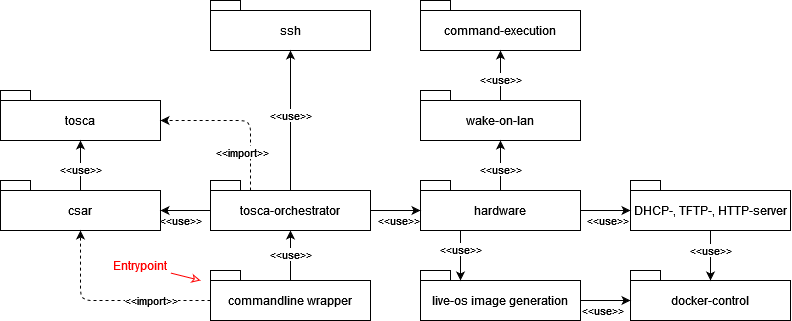
\includegraphics[width=14cm]{packages}
  \centering
  \caption{UML package diagram describing how the packages are related to each other}
  \label{image:packages}
\end{figure}

As can be seen in the diagram, the commandline-wrapper communicates only with one package: The orchestrator, which does all of the actual work. For non-bare-metal applications, the orchestrator only uses the \gls{csaracr}, the \gls{sshacr}, and the command-execution package directly. They are sufficient to be compliant with the current standard specification. When bare-metal machines should be provisioned, the orchestrator also communicates with the hardware package. It manages the generation of the live-\gls{osacr} image, the interactions with the \gls{dhcpacr}-, \gls{tftpacr}-, and \gls{httpacr}-servers, as well as the wake-process of the bare-metal machines.
\newline
When invoked with the initialization subcommand, the application assumes hardware will be provisioned and generates the necessary artifacts.
\newline
Deployment of applications starts with parsing the \gls{csaracr} contents. While the \gls{csaracr} package handles file-I/O, the \gls{toscaacr} package is the actual parser.

\subsection{TOSCA}
In order to be able to implement a library for the \gls{toscaacr} standard, it is necessary to work through both the original specification and the Simple-Profile extension counterpart, since both are meant to work together. Important information is sometimes distributed over both specifications, so to fully understand it, this is necessary. Additionally, preexisting libraries for the chosen programming language might exist. In case of this thesis' reference implementation Golang is the language of choice. Sadly, most of the larger libraries are based on one another or unfinished, and the most complete of them are severly outdated \cite{github_toscalib_forks}.
\newline
In order to support the latest version of the specification, and to be able to easily extend it if necessary, a complete reimplementation of the \gls{toscaacr} library is created. It is strongly influenced by the largest but outdated one, but is more complete. Only with the already described line-by-line read-through of both specifications it is possible to gather enough information about the standard and all its features.
\newline
With the new library, it is possible to parse any (valid) Types, Templates, and Service Topologies.
In addition to parsing them and creating Go-native structures out of them, basic functions like \textquote{get\_input} and \textquote{get\_attribute} or validation of elements, it is limited to one implementation type, Bash, while the specification states that Python should be supported as well. This is due to the proof-of-concept nature of this thesis. Sadly, there are several occasions in the specifications, where it is unclear or simply incomplete. These cases are mostly about edge cases and were not required for the proof-of-concept this thesis tries to achieve. Therefore, they were left out of the implementation. Other cases, such as inconsistencies or required assumptions will be covered in the chapter \textquote{Analysis}.
\newline
Because the basic \gls{toscaacr} specification describes how to work with extensions like the \gls{toscaacr} Simple Profile, it is possible to implement such imports, references, and relations as well. This means, the implemented \gls{toscaacr} library (called package in Golang context) is fully compatible with the \gls{toscaacr} Simple Profile and all other extensions.
\newline
The package is also meant to solve the type derivation, resolve imports, namespacing and validate all of them.

%TODO add TOSCA processor, orchestrator etc definitions, and what is fulfilled or not

% TODO describe public functions (all packages)

\subsection{CSAR}
After the \gls{toscaacr} package is able to parse the contents of files, the file-I/O - desribed in the last chapter of the specification -  is implemented as a seperate package. It contains information about how to pack multiple artifacts like \gls{osacr}-images, definition-, or other required files together into one CSAR file. The file is basically a standard zip-archive, but the content needs to follow a certain schema. For example there are three places where required metadata like version and name can be placed. If they are not found there, the whole file is invalid.
\newline
The reason behind this seperation are the still very different domains: The \gls{toscaacr} package parses file contents and provides Go-native types, while the \gls{csaracr} package is more about accessing files, checking for their existance and making it possible for the \gls{toscaacr} package to parse its content. Should another project work with filecontents in a database for example, they would not require the file handling and can import only the \gls{toscaacr} package.
\newline
This package depends on the earlier described \gls{toscaacr} one, as it has a function that takes a file-/folderpath as input and returns the fully parsed \gls{toscaacr} topology with fully derived templates. \textquote{Fully derived} means that all imports are made and template properties are extended with values from their original type wherever necessary.

%TODO describe public functions

\subsection{Command-execution}
In order to run Bash commands from the application itself and retrieve the outputs, it makes sense to build a complete package around command execution. It can later be extended with a corresponding implementation for Python, so the application is fully compatible to the \gls{toscaacr} specification.
\newline
The package provides to public methods. One for running direct commands, and another for running a script that resides at a provided location.
\newline
Since \gls{toscaacr} only introduces Bash and Python, this package requires the underlying system to be compatible with both script languages. Windows for example does not support Bash by default.

\subsection{Docker control}
It is clear that some kind of \gls{dhcpacr}- and \gls{tftpacr}-server is required. They could be external applications, but it should not be a hard requirement. In cases where no external \gls{dhcpacr}- and \gls{tftpacr}-servers exist, it must be possible to set them up in an easily repeatable way. The same applies to the generation of the live-\gls{osacr} image. As in most such cases, this can be solved with (docker) containers. The goal of this thesis is to bring all required bits together, so the application needs to create the docker images, start the containers (with parameters like volumes and forwarded ports), as well as stop and remove the containers when they are not needed anymore (for example when the provisioning is finished).
\newline
The official docker binary (for Linux) is created in Golang as well, and the software is open source. Docker even provides an SDK for other developers to integrate communication with the docker engine into their applications.
Sadly, the documentation is sparse and the few examples shown along the SDK are often not enough to get even seemingly easy things like container stopping to work. For this particular case it is necessary to add the container stopping and removal twice: Once, when the application terminates successfully, as the container fulfilled its job and isn't needed any more. And a second time, when the application terminates due to an error somewhere else, and the default termination does not happen. Even \textquote{deferring} the container termination does not work. Only when the SIGTERM interrupt of the wrapper application is \textquote{manually} listended for and a function is implemented to remove the container in such a case, the removal is successfull in all cases.
\newline
Another obstacle is the retrieval of live logs during the container livecycle and embed the retrieved output in the logs of the wrapping application. This can be solved by creating a buffered streamreader, which is periodically polled and checked for contained linebreaks.
\newline
As the application is now able to handle docker containers to provide repeatable setup of the DHCP- and TFTP-server, the next step is to implement a repeatable way of a live-\gls{osacr} image generation.

\subsection{Live-OS image generation}
The huge amount of time needed to install a complete \gls{osacr} just for retrieving information about the hardware has the potential to be a huge showstopper. In order to reduce the time needed for information retrieval, a live operating system is used. These operating systems are not necessarily very different from normal ones, but they can most often run from read-only mediums like optical disks. Examples are all \gls{osacr} installers (that can be burned to CD-ROM or similar) - this means there already are many live systems out there.
\newline
Since the live-\gls{osacr} is provided via network, a virtual version of such a system is required. One such file-format for disk images is defined by the ISO 9660 standard \cite{iso9660_spec}. The extension of these files is either \mintinline[bgcolor=lightgray,breaklines]{bash}{.iso} or \mintinline[bgcolor=lightgray,breaklines]{bash}{.udf}. Due to the name of both the standard and the extension, these files are often simply called iso-files.
\newline
In order to be able to create a iso-file that provides information about the underlying hardware from scratch, only one requirement should exists: A working internet connection. Optimally, a generic preexisting live-image is downloaded and then modified to serve the special use case of publishing the desired information. Since tiny Linux images should be relatively common in times of Internet-of-Things and Raspberry Pis, this should be an easy task. The experience tells a different story, though.
\newline
The first linux distribution tested during the implementation phase was \textquote{Minimal Linux Live}. It is described as an educational Linux, so its configuration is well-documented \cite{mll}. A first test with the original downloaded iso file seemed promising: The filesize is less than 50 MB, the \gls{osacr} boots in under 30 seconds and the due to its educational background, it is easily extensible. When the system is fully up and running, the keyboard (mouse is not supported) input did not work under the tested Hyper-V hypervisor. As this is not exactly necessary, the image generation was extended in such a way, that a webserver is started when the system boots. But with or without this extension, the generated image is not bootable on said hypervisor. Tested were both \gls{biosacr} and \gls{uefiacr} firmwares - to no avail.
\newline
A second promising \gls{osacr} is Alpine Linux. It is a full-blown operating system with focus on small footprint and a fast boot process. Due to its focus, it is very widespread in the container world, and its documentation is extremely good. There is even a dedicated wiki-page for custom iso-images \cite{alpine_custom_iso}. Since there are additional applications necessary to be installed in order to generate the image, and these applications are installed with the Alpine Linux package management tool \textquote{apk}, the first test was run in an Alpine-docker-container. Later, the same things were tested with an Alpine-\gls{vmacr}, with the same result. The generated iso-image is four times the size of the original downloadable alpine iso. Not only is there a huge size difference, but when trying to boot it, a kernel file is not found. As described earlier, the overall documentation is quite good, and there are several predefined build-profiles for custom images. While the size is different for each one, the kernel file issue reoccurs in all cases. Even when inserting the missing file from the original Alpine iso, the generated iso remains unbootable.
\newline
Another Linux distribution with good documentation and widespread use is Ubuntu. In the Ubuntu app store, there exists a complete graphical application dedicated to image generation. It works perfectly, and the concept with an autostarted webserver that serves information about the underlying hardware can be considered proven. But since the size of the iso file exceeds one GB, and the boot time is close to one minute, another well-known operating system was tried.
\newline
Due to slower release cycles, Debian is considered more stable than Ubuntu. At the same time it has not as many features (preinstalled). Therefore its initial size is significantly lower and its non-teaked performance is generally better. While for custom Debian images there is no graphical tool, the Ubuntu one shows the general approach. The steps can be summarized as follows:

\begin{enumerate}
  \item Unpack the original iso file.
  \item Unpack the contained filesystem-image (squashfs).
  \item Simulate a running operating system on the unpacked contents with \mintinline[bgcolor=lightgray,breaklines]{bash}{chroot}.
  \item Make all necessary changes, like installing applications, enable services and adding files. This can include boot-menu adjustments like reducing/removing the timeout.
  \item Repack the filesystem-image.
  \item Repack the image with the changed filesystem-image.
\end{enumerate}

The resulting image is smaller than one GB, boots in under ten seconds, is as extensible as the Ubuntu image, and due to its textual nature completey scriptable. Especially the last part makes it the perfect fit for putting it in a container. It is therefore the selected way to generate a live-\gls{osacr} image.
\newline
The customizations include a webserver that autostarts during boot, and a simple service that also starts automatically during the boot-process. The service runs some commands and stores the output into files that are then served by the webserver. Due to the proof-of-concept nature, only information about the CPU and RAM is served.

\subsection{DHCP-, TFTP-, HTTP-server}
The \gls{dhcpacr}-server does not only provide devices with (temporary) IP-addresses, but additional information about the network as well. Common examples are the subnet mask and the network gateway for routing beyond the current network. But the \gls{dhcpacr}-server can advertise options for network-boot as well. This includes the URL of a boot firmware on a \gls{tftpacr}-server. Since \gls{biosacr} and \gls{uefiacr} require different files there, a condition is required to run on the \gls{dhcpacr}-server. As described earlier, \gls{tftpacr} is not very efficient, and to support \gls{httpacr}, a boot firmware named iPXE is distributed and loaded before the actual operating system. The loaded iPXE will then send another \gls{dhcpacr} request and will as a result begin to load iPXE anew. To escape this loop, the DHCP-server can detect whether the client is iPXE or not. In case it is not, the iPXE firmware for this specific client is provided (as described above). In case it is, a script location is passed. This can be a simple \gls{httpacr} URL. The \gls{httpacr}-server can then dynamically provide the client with special iPXE-instructions and the actual live-\gls{osacr} image.
\newline
The software dnsmasq combines \gls{dhcpacr} and \gls{tftpacr} server (DNS as well, but that is not needed here). In order to start and stop the servers on-demand and in one go, dnsmasq and a webserver of choice is installed in a container image. When running the container, the hostport 67 (UDP) is required for \gls{dhcpacr}-, hostport 69 (UDP) for \gls{tftpacr}-, and hostport 80 (TCP) for the \gls{httpacr}-server. The previously generated live-\gls{osacr} image is provided as a volume mount.

% docker container, ports, variable config vs fixed config
% why not external ones

\subsection{Wake-on-lan}
In order to wake a machine, a so-called magic packet is broadcasted. This packet has a very special format. The only \textquote{real} payload is the MAC-address of the \gls{nicacr} that can power the attached machine when the packet is received.
\newline
This package contains methods for the creation and broadcasting of the magic packet for a MAC-address. Since \gls{wolacr} is incompatible with most hypervisors, an additional mechanism has to check whether a hypervisor hosts a \gls{vmacr} with the specified MAC-address. Should this be the case, it determines its identifier and issues the hypervisor to power the \gls{vmacr} on.

\subsection{Hardware}
The hardware package manages the bare metal provisioning process. It controls the container that is responsible for the \gls{dhcpacr}-, \gls{tftpacr}- and \gls{httpacr}-servers. It also initiates live-\gls{osacr} image generation. And it issues the calls to the wake-on-lan package. Because the loading and booting of the live-\gls{osacr} still takes several seconds, a simple \gls{httpacr} request would time out and the provisioning would fail. Therefore, this package also waits until the hardware information is available. Because of the lease time of issued IP-addresses, the \gls{dhcpacr}-server assigns different IP-addresses to a machine that wants to boot via network and when the live-\gls{osacr} comes up. The hardware package therefore also checks the lease-list of the \gls{dhcpacr}-server for the latest IP-address for each MAC-address.
\newline
Upon having gathered all desired information about the hardware, the package returns the information to the orchestrator package.

\subsection{SSH}
%TODO add sources and text on why password auth is bad
In order to provide the most possible security for deployed live-\gls{osacr} images, \gls{sshacr} password authentication is disabled. To run remote commands, an \gls{sshacr} public key is included in the image generation workflow. This package manages the generation of a public/private key-pair, as well as invoking commands on the remote machines. In case of the latter, it returns the output to the orchestrator for further processing (like logging).

% TODO Why only manipulate live-os, instead of deploying complete new os
